\chapter{Appendix B: The 
% ukr\_pravda\_titles\_2y 
UKR-RUS-ENG Ukrainska Pravda dataset}\label{app:pravda}

\section{Basics}
This section describes the collection of \textit{ukr\_pravda\_titles\_2y}\footnote{\href{https://huggingface.co/datasets/shamotskyi/ukr_pravda_2y}{https://huggingface.co/datasets/shamotskyi/ukr\_pravda\_2y}}, the dataset 
from which UP-Titles was built.
The crawler used to collect it, \textit{UPCrawler}\footnote{\href{https://github.com/pchr8/up_crawler}{https://github.com/pchr8/up\_crawler}},
is released under the MIT license.

\section{Description}
The dataset contains articles published from the 01.01.2022 to 31.12.2023, since UP drastically increased the amount of articles translated to English after the start of the full-scale invasion on the 24.02.2022.
The UPravda multilingual dataset contains in total \textbf{145,520} articles in all languages, of them \textbf{55,338} in Ukrainian, \textbf{55,231} in Russian, and \textbf{34,951} in English. Most of them aren't original articles but translations, e.g. the same article can be found once in Ukrainian and once in Russian. A chronological distribution is shown on \autoref{fig:up_languages}.
The dataset has \textbf{1,390} individual tags.

\begin{figure}[ht]
    \centering
    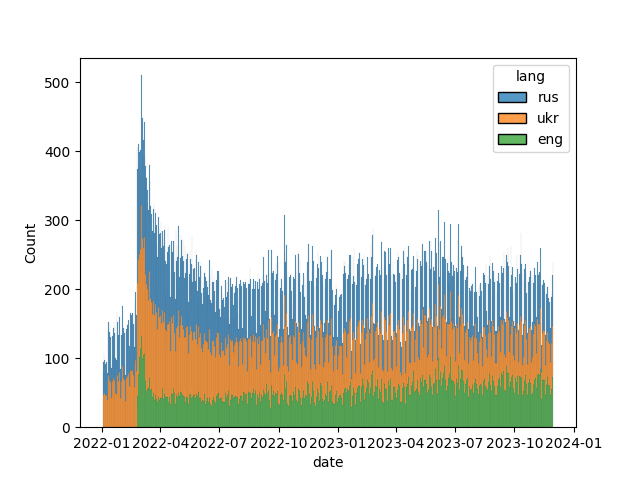
\includegraphics[width=0.8\textwidth]{Figures/up_ds_langs.png}
    \caption[Language distribution of the ukr\_pravda\_2y dataset]{Language distribution of the dataset; note the sudden increase of both Russian and English articles (mostly translations) at the start of the invasion the 24.02.2022.}
    \label{fig:up_languages}
\end{figure}


\section{Dataset collection}
\label{sec:up-titles-collection}

% The dataset is released on the HF Hub at \href{https://huggingface.co/datasets/shamotskyi/ukr_pravda_2y}{https://huggingface.co/datasets/shamotskyi/ukr_pravda_2y} / doi \href{https://doi.org/10.57967/hf/1476}{https://doi.org/10.57967/hf/1476} under the \href{https://creativecommons.org/licenses/by-nc/4.0/}{CC BY-NC 4.0} license.

\subsection{Ukrainska Pravda}
Ukrainska Pravda\footnote{\href{https://www.pravda.com.ua/}{https://www.pravda.com.ua/}} 
(lit. ``Ukrainian Truth'')
is a Ukrainian online newspaper for a general readership writing, mostly, about political and social topics.

% In 2017, it was in the eighth most cited source of the Ukrainian Wikipedia\footnote{TODO - better source} and in 2020 it was the most visited online news website in Ukraine\footnote{TODO - better source}. The Institute of Mass Information listed Ukrainska Pravda among the six online editions with the highest level of compliance with professional journalistic standards in 2021.

\subsection{Website structure}

UP (Ukrainska Pravda) publishes articles predominantly in Ukrainian, with some being translated to Russian and English. Each article can belong to zero or more ``topics'' (tags) that are mostly preserved across translations.
Each article has an article ID that is constant across translations.

\subsection{Crawling}

The CLI interface expects a date range (using natural language, e.g. ``last year'') and a target folder, where the pages are saved.   

\begin{figure}[ht]
    \centering
    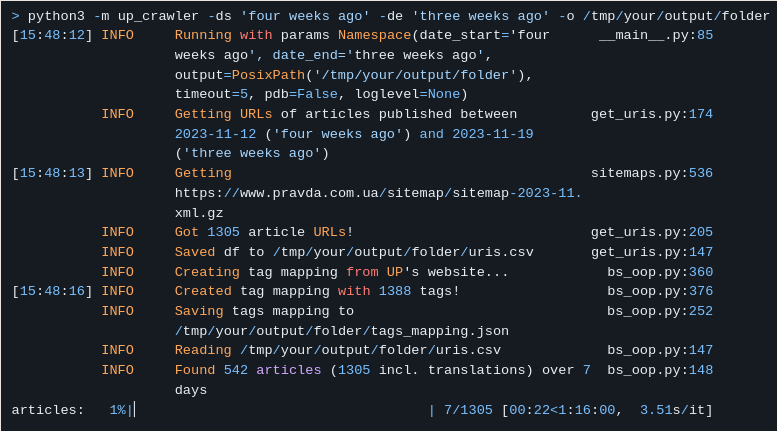
\includegraphics[width=1.0\textwidth]{Figures/2024-04-14-021138_777x431_scrot.png}
    \caption{The UPCrawler interface.}
    \label{fig:crawler}
\end{figure}

The package parses the XML sitemaps using the \textit{advertools}\footnote{\href{https://pypi.org/project/advertools/}{https://pypi.org/project/advertools/}} Python package.
% Initially, the package \texttt{UPCrawler} used the daily archive pages (e.g. \url{https://www.pravda.com.ua/archives/date_27092023/}) to get the URLs of articles published on a specific day, then for each article URL accessed the expected locations of the Russian and English translations to check if a translation exists. Later, I rewrote the code to use a much better solution: parsing the XML sitemaps (e.g. \url{https://www.pravda.com.ua/sitemap/sitemap-2023-09.xml.gz}) using the \href{https://pypi.org/project/advertools/}{advertools} Python package.
% \textbf{Sitemaps}\footnote{Schonfeld, 2009} is an XML-based protocol used to inform search engines about the URLs available for web crawling, as well as provide additional information about it such as when was the page last updated, how often does the content change, etc.

% The following regex (see \url{https://regex101.com/r/dYlIiF/4} for an interactive analysis) is used to parse each URL to get the language of the article, the article ID, the section (news, podcasts, ..) etc.:

% \begin{verbatim}
% URI_REGEX_STR_EXT = r"(?P<uri>(?P<domain>.*\.com\.ua\/)(?P<lang>(eng)|(rus))?\/?(...
% \end{verbatim}

Crawling the articles is done using the \textit{beautifulsoup4}\footnote{\href{https://pypi.org/project/beautifulsoup4/}{https://pypi.org/project/beautifulsoup4/}}
library. 
The alternative option of using the \textit{newspaper3k}\footnote{\href{https://newspaper.readthedocs.io}{https://newspaper.readthedocs.io}}
package was also considered, it was able to detect the article, title, and metadata from UP surprisingly well, but it incorrectly detected some fields (which would have required manual fixes anyway), so the existing from-scratch implementation was kept.

For transparency and in the spirit of ethical crawling, there were timeouts between requests, and the unique user agent contained a short explanation of the Thesis project as well as a contact email. The email address was never used, and the crawler was never blocked.

\section{Dataset construction}
% The article text inside \texttt{<article>} was taken from each page. The content of the tags \texttt{<p>} and \texttt{<li>} were used to extract the plaintext while avoiding advertisements, infoboxes etc.

Paragraphs matching some standard article endings like ``follow us on Twitter'' were excluded from the article texts, but not all such endings were covered.
The tags required special care because they presented two problems:
\begin{enumerate}
    \tightlist
    \item There were pages with lists of tags in Ukrainian and Russian but not English.
    \item Some tags had translations to other languages, some didn't.
\end{enumerate}
Since this was supposed to be a multilingual dataset a list of tags for each article, independent of the translations, would have been a strong asset.
The solution at the end was to crawl Ukrainian and Russian tags pages to save the short unique ID and both translations, then add English translations to the short IDs when they were first encountered.

An example tag and three translations:
\begin{minted}{json}
{
    "ukr":["флот","/tags/flot/"],
    "rus":["флот","/rus/tags/flot/"],
    "eng":["naval fleet","/eng/tags/flot/"]
}
\end{minted}

\section{Mitigations of issues found in multilingual datasets}

A recent (2022) manual audit of available crawled multilingual datasets~\cite{10.1162/tacl_a_00447} found surprisingly low amounts of in-language data and systematic issues in many of them. Some issues raised in the paper relevant to this dataset include:
\begin{itemize}
\tightlist
    \item Using standard unambiguous ISO 639-3 language codes (ukr, rus, eng). ISO 639-3 was chosen instead of the more common ISO 639-1 (uk, ru, en) because of the possibly ambiguous `uk' that can be associated with Great Britain as well. Interestingly, the more familiar `UA' is a valid ISO code for the country, but not the language.
    \item The language identification was performed from the URL of the page (in turn labeled by UP), not through automated language identification processes (especially relevant in light of the ukr/rus disambiguation issues common in many Ukrainian datasets, e.g. as seen in GRAC~\cite{9648705}).
    \item The texts themselves were written by proficient language users, not automated translations.
    \item The dataset is digital-first: no errors were introduced by OCR, incorrect layout parsing etc.
    \item Manual spot-checks of random articles were done to ascertain the different translations are indeed 1) text, 2) in the stated languages, 3) and actually refer to the same article.
\end{itemize}

\section{Licensing}
According to Ukrainian law, newspaper-like articles aren't subject to copyright. According to UP's rules on the matter, reprinting in other online-newspapers is free but requires a link to the UP article not later than the second paragraph. Using the materials for commercial reasons is forbidden.

Releasing this dataset under the \href{https://creativecommons.org/licenses/by-nc/4.0/}{CC BY-NC 4.0} license (that allows sharing and adaptation only with attribution and for non-commercial use), with clear attribution to UP in the name and the description of the dataset, fulfills the applicable obligations both in letter and in spirit.

% The dataset is released at \url{https://huggingface.co/datasets/shamotskyi/ukr_pravda_2y}

% \subsubsection{Similar datasets}

% \begin{itemize}
%     \item \href{https://fido-ai.github.io/ua-datasets/examples/ua_news/}{UA News classification - ua-datasets}
%     \item \href{https://huggingface.co/datasets/Yehor/ukrainian-news-headlines}{Yehor/ukrainian-news-headlines · Datasets at Hugging Face}
%     \item \href{https://huggingface.co/datasets/zeusfsx/ukrainian-news}{zeusfsx/ukrainian-news · Datasets at Hugging Face}
% \end{itemize}
